\documentclass[12pt]{article}

\usepackage{fullpage}
\usepackage{multicol,multirow}
\usepackage{tabularx}
\usepackage{ulem}
\usepackage[utf8]{inputenc}
\usepackage[russian]{babel}
\usepackage{graphicx}
\usepackage{indentfirst}


\begin{document}

\section*{Лабораторная работа №\,2 по курсу дискрeтного анализа: сортировка за линейное время}

Выполнил студент группы М08-207Б МАИ \textit{Цапков Александр}.

\subsection*{Условие}

\begin{enumerate}
\item Вариант №04

Необходимо создать программную библиотеку, реализующую указанную структуру данных, на основе которой разработать программу-словарь. В словаре каждому ключу, представляющему из себя регистронезависимую последовательность букв английского алфавита длиной не более 256 символов, поставлен в соответствие некоторый номер, от 0 до 264 - 1. Разным словам может быть поставлен в соответствие один и тот же номер.
\item B-Tree.
 
\end{enumerate}

\subsection*{Метод решения}

В моем варианте лабараторной мне нужно реализовать словарь используя стуктуру дерева B-Дерево. Эта стуктура отличается от остальных тем, что с помощью параметра дерева (T) можно контролировать его высоту и ширину. Это было придумано для того, чтобы уменьшить именно высоту, так как при больших размерах нодов гораздо более затратной операцией вляется именно загрузка и выгрузка этого нода в и из оперативной памяти. Таким образом при большом T происходит меньшее количество работы с жестким диском. 

Устроена структура следующим образом: в каждом ноде может быть от T - 1 до 2T - 1  элементов, за тем лишь сключением, что в корне дерева нет ограничения снизу. Все элементы в узлах отсортированы по ключу. У каждого ключа есть ссылка на правый и на левый от него нод, причем правая ссылка элемента равна левой следующего и все ключи узла по этой ссылке находятся в диапазоне между ключами этих 2-х элементов. Таким образом у каждого нода  N + 1 ссылка на дочерние узлы, где N это количество жэлементов в искомом узле. Прелесть B-Дкрева состоит в том, что высота всех его листов всегда одинаковая.  

\subsection*{Описание программы}

Для реализации своего дерева я решил воспользоваться списками. Решение это было принято из тех соображений, что при добавлении нового элемента в дерево и удалении из него приходится перемещать целые блоки элементов из одного узла в другой. При использовании списков я могу перемещать только ссылки на узлы списка, пересвязывать их и менять головы и хвосты, что ускоряет реструктуризацию дерева и предотвращает лишнее копирование элементов. Класс TKeyVal содержит в себе 3 поля: ключ, значение и ссылку на левый элемент. Таким образом для хранения N  элементов приходится использовать N + 1 узел списка для того чтобы хранить правую ссылку крайнего элемента с права. В остальном дерево реализовано точно по алгориму. 

Из особенностей я реализовал свою структуру с использованием шаблона, и поэтому ее можно использовать с другими ключами, поддерживающими операции сравнения и присваивания. Я же, так как нельзя использзовать стандартные контейнеры, реализовал свой класс строк со всеми операциями сравнения, но в отличие от стандартного string моя реализованна на статике (267 символов максимум).

Источник: внимательно слушал Никиту Константиновича Макарова на лекциях.

\subsection*{Дневник отладки}

1-6 Попытки: неправильный ответ и ошибки выполнения на 1 2 и 6 тестах. Справлял вставку и удаление, не было функций загрузки и сохранения дерева. Исправил ввод в свою строку что ускорило программу в 3-4 раза.

7 Попытка: Добавил функции сохранения и загрузки. Ошибка валгрина на запись неинициализированных символов. Добавил их иничиализацию в конструктор своей строки

8-N Попыток: Превышено время выполнения. Присутствовали лишние копирования, писал операторы перемещения, заменил свое сравнение строк на strcmp. В после некоторых "оптимизаций" программа стала даже медленние и я откатывался к предыдущим вариантам. 

1 Попытка на 2-м аккаунте: До сих пор превышено время, но код ускорился на 10-20 сек с начала оптимизации. Запустил профайлер и узнал что все время идет на очень неэффективный ввод строки. Заменил на обычный cin с приведением к маленьким буквам в цикле.
2 Попытка на 2-м аккаунте: Прошло все тесты.

\subsection*{Тест производительности}
Для проверки скорости программы я воспользовался скриптом который генерирует тесты, проверяет скорость работы на разном их 
количестве и сам строит график. По графику можно убедится что сложность операций действительно логарифмическая.

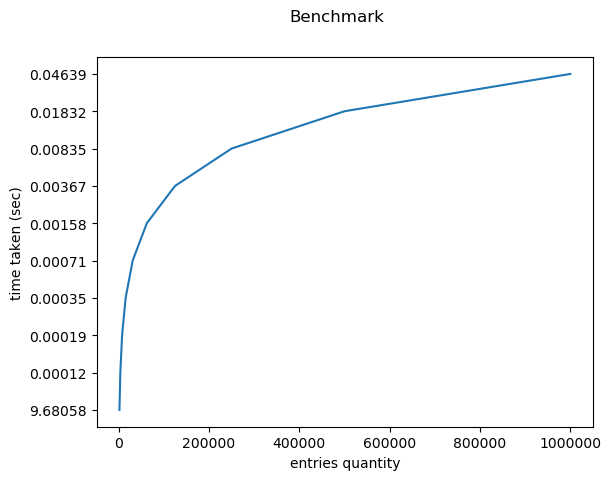
\includegraphics[width=\linewidth]{benchmark}

\subsection*{Выводы}

После этой ЛР я получил хорошо работающее B-Дерево на шаблонах, которое я могу использовать в других своих работах. Но использование тменно этоц реализации не раскрывает всех плюсов б дерева так как нет загрузки и выгрузки узлов из памяти компютера и обычные красно черное дерево или AVL  были бы больше к месту. Еще я понял что для такой большой работы необходими пользоваться всеми предоставленными программисту инструментами, такими как отладчики и профайлеры, без них моя работа заняла бы гораздо больше времени.

\end{document}

